\section{The adventure game} \label{adventureGame}
In our work with the CLS we have been working on creating an adventure game where the CLS would allow us to create different variations of the game based on the repository of code we have built. We have not built the game from the ground up, but instead we have taken a demo project from the Orleans documentation \cite{AdventureGame} and extended it. This was done to save development time and thus to reach a point where we could begin creating combinators faster and have a more 'real world'-like system to work with. The original system involved players, monsters and rooms where all players and monsters would have one health. Things or items were scattered across the rooms and the players could pick them up. Most noticeably is the knife which allows a player to stab other players or monsters. The players and monsters could then move around the rooms, but the monsters would never attack. The game had no objective and no way to win. It served as a 'sandbox' project. There were other smaller implementations which were part of the original game, but because these have little to no relevance to our project we will leave them out of this overview.\\
The first extension to the game was the addition of health for both the players and monsters. This allowed us to interact in a more fine grained manner with the monsters, and opened up the possibilities of adding abilities to the player. We also extended the monster such that it would attack the players. These two additions makes our foundation for the game, and is what we would like to call our \textit{initial application} as everything else we have created revolves around this foundation.\\

With our extensions the game still has no objective. Our extensions have served only to show the use of the CLS tool to create and test actor code. The game is thus still a sandbox and can not be won.\\
We have extended the player with two abilities. The first is a fireball which deals high damage. The other ability is a roar which makes the player take half damage and healing for ten seconds. Both abilities have a cooldown (time before the ability can be used again). The idea is, the player has either the fireball ability, the roar ability or neither, and that we achieve this through use of the CLS.\\
The boss is an extension entirely created by us. The boss is a strong enemy which can spawn small monsters and has a lot of health. Further we have created two abilities for it, one which heals all spawned monsters in the room, and one where the boss takes half damage if there are spawned monsters in the room with it. Again the idea is, through the use of CLS the boss either has one of the two abilities or is not in the game at all.\\
The room has been extended with weather effects. We have created four different weather effects which affects players differently every time they enter a room. We have \textit{blizzard} which deals five damage to the player. \textit{Sunny} which heals the player for ten health. \textit{Cloudy} which does nothing and \textit{night} which makes it so the player gets fewer details about the room when it enters. The idea is that a random weather from a pool of available weathers (we get to this in \autoref{Metalanguage}) is chosen each time the player enters a room.
\begin{figure}[H]
	\centering
	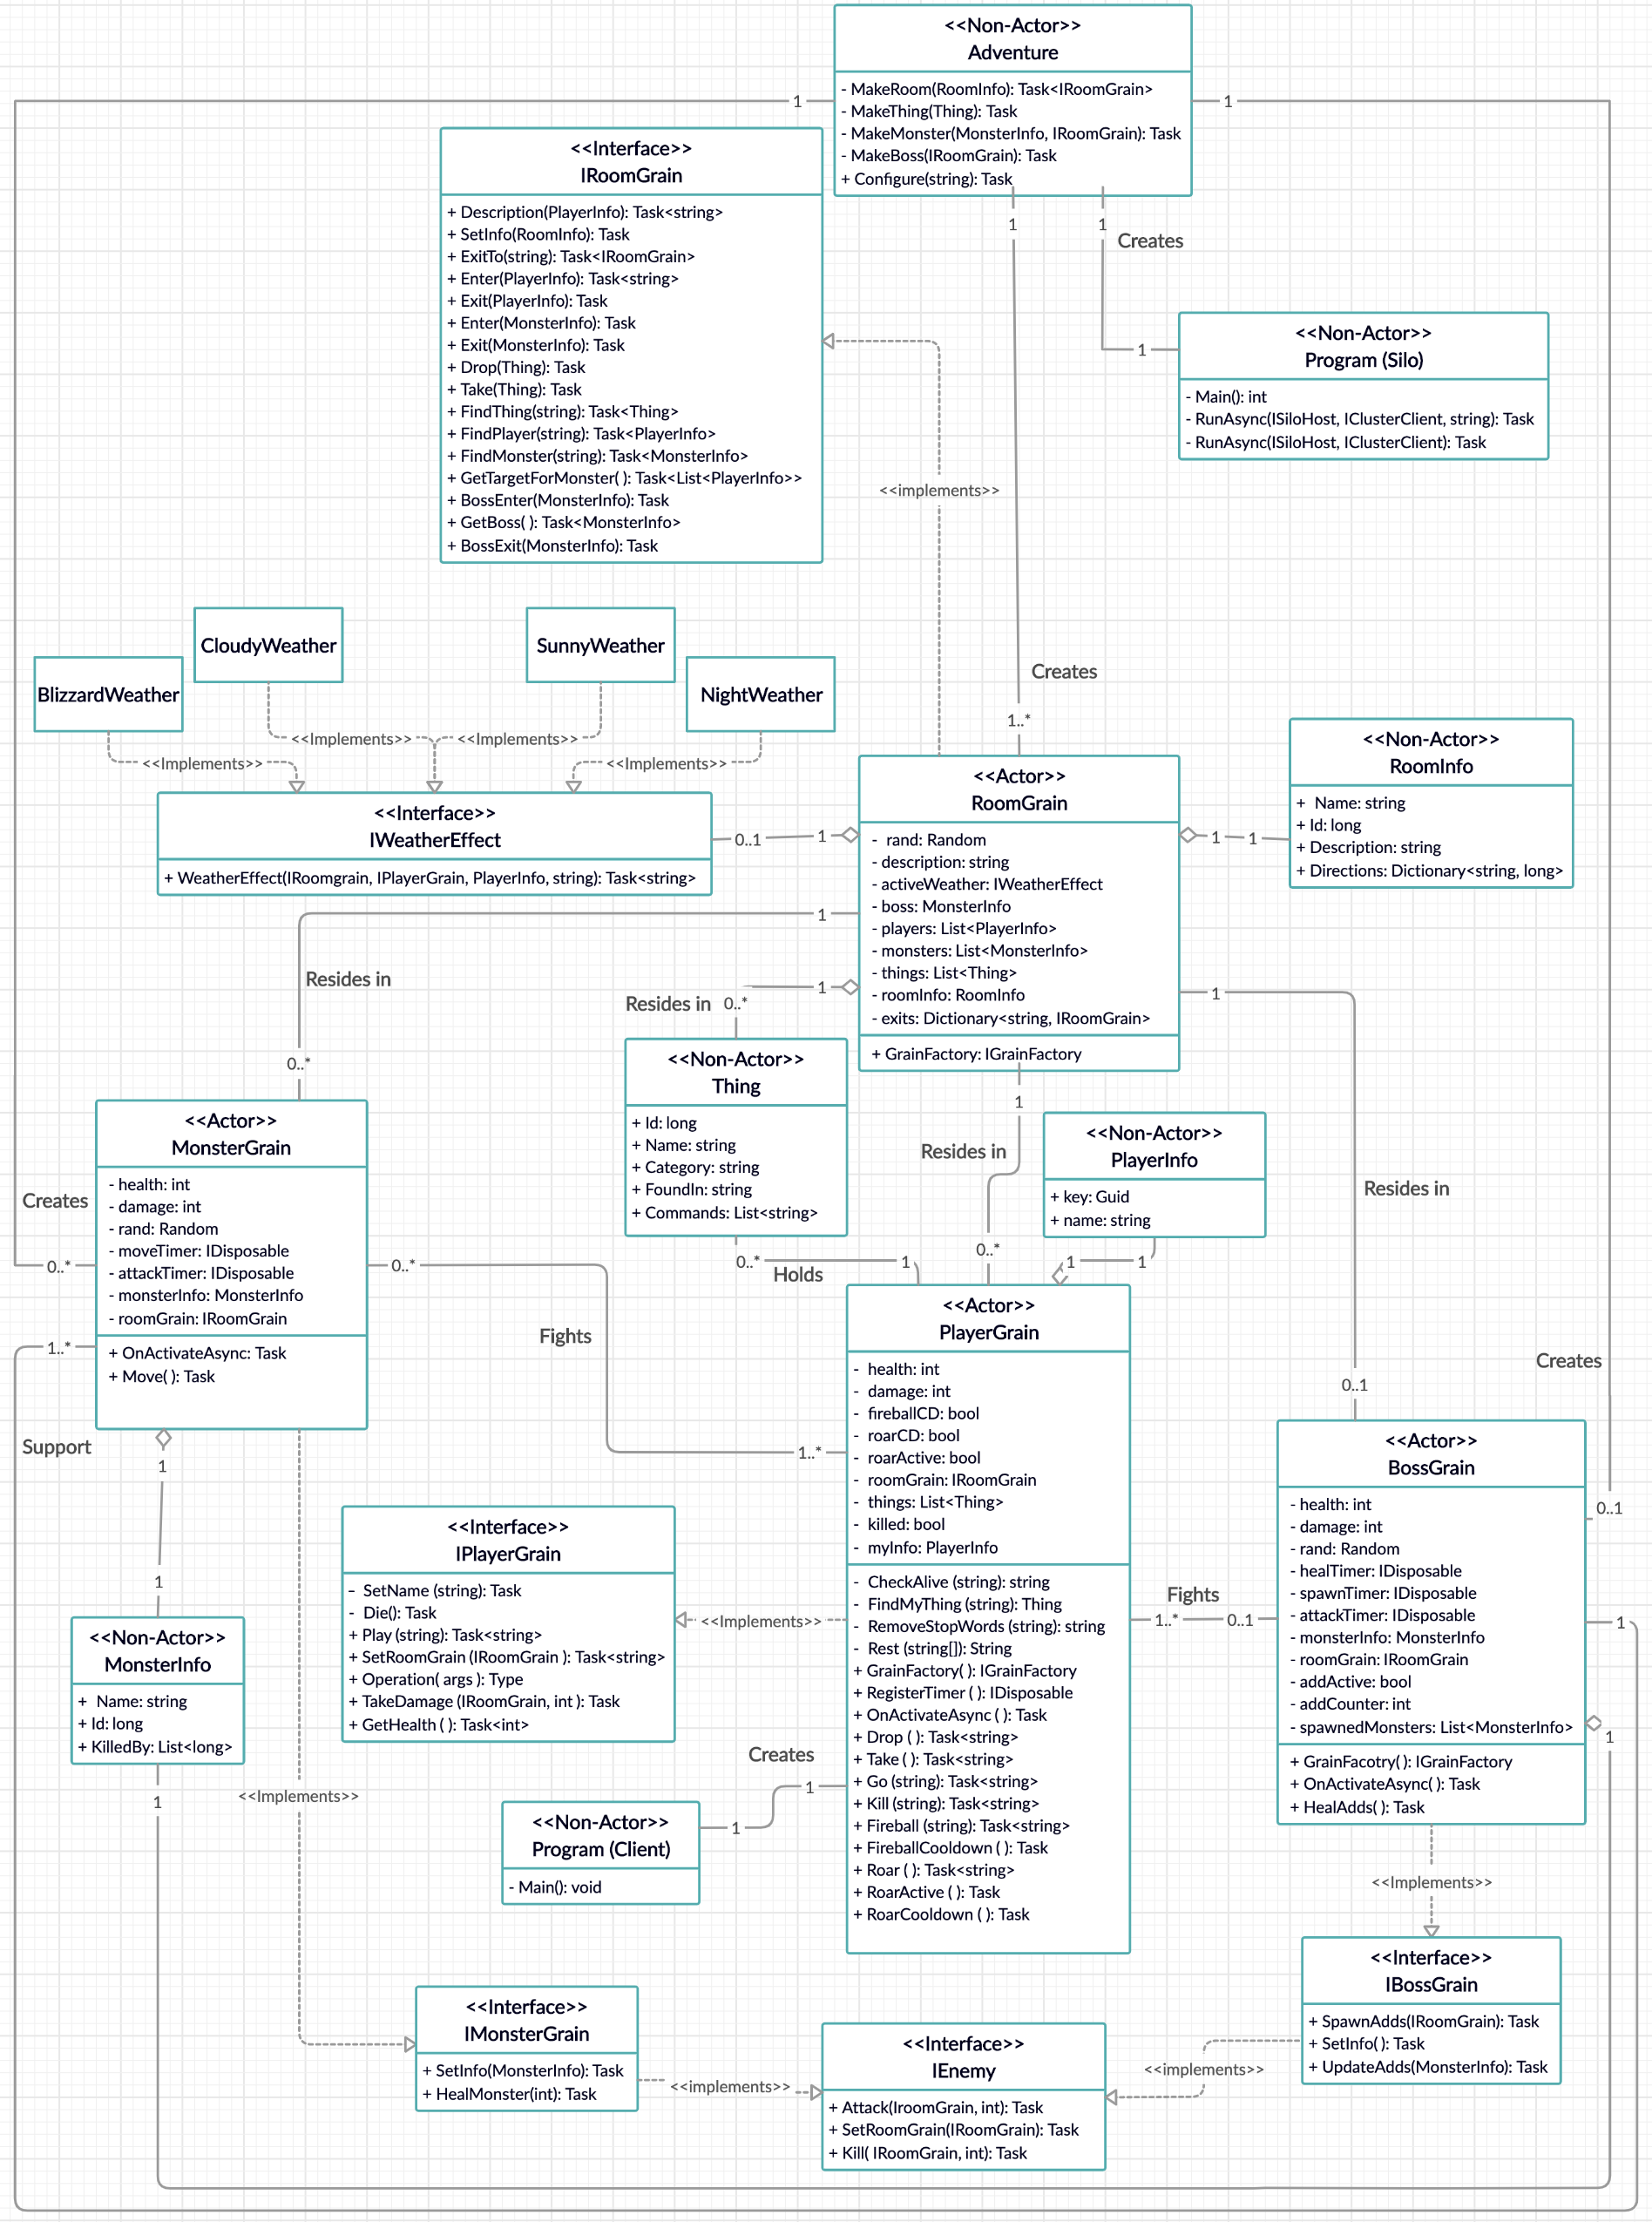
\includegraphics[width=\linewidth]{Materials/Adventuregame/ClassDiagram}
	\caption{UML class diagram of the adventure game with all extensions available.}
	\label{UML}
\end{figure}
In \autoref{UML} we see an UML class diagram for the whole game with all extensions. We see that there is quite high coupling between the room and the other actors, and in general a lot of communication the actors in-between. The room object works as a mediator object, and holds information about everyone in the room. The other objects do not know of each other, but instead asks the room if a player or specific monster is in the room with them. Because of this, the room will receive a lot of communication as for all tasks involving more than one actor, the room will be prompted. However, as there are a lot of rooms, we can not talk about a bottleneck. If we were to scale the game with a lot of players and monsters, we would likely scale the number of rooms proportionally, and so there will not be a lot of communication to one specific instantiation. In addition, the communication with the room is in general short, for instance when a player wants to fireball a monster. In \autoref{PLayerFireballFlow} we see a sequence diagram of a player using fireball on a monster. The player first asks the room to find players of the target's name, as there are none, the player then asks for monsters of the same name. This time there is one and the player can then tell the monster to take damage. As we see, these lookups are only calls to a single function, and thus the communication is short.\\
If we look at the communication between the boss and the monsters it is only one way. The boss holds its own list of monsters it has spawned and thus does not need to prompt the room for what monsters are present. The room does however communicate to the boss when a monster dies in the room such that it can update its list. The boss can now go through its list of monsters and for each one tell it to heal. The boss does only have communication with monsters it spawns, not with the monsters found around the world.\\

\begin{figure}[H]
	\centering
	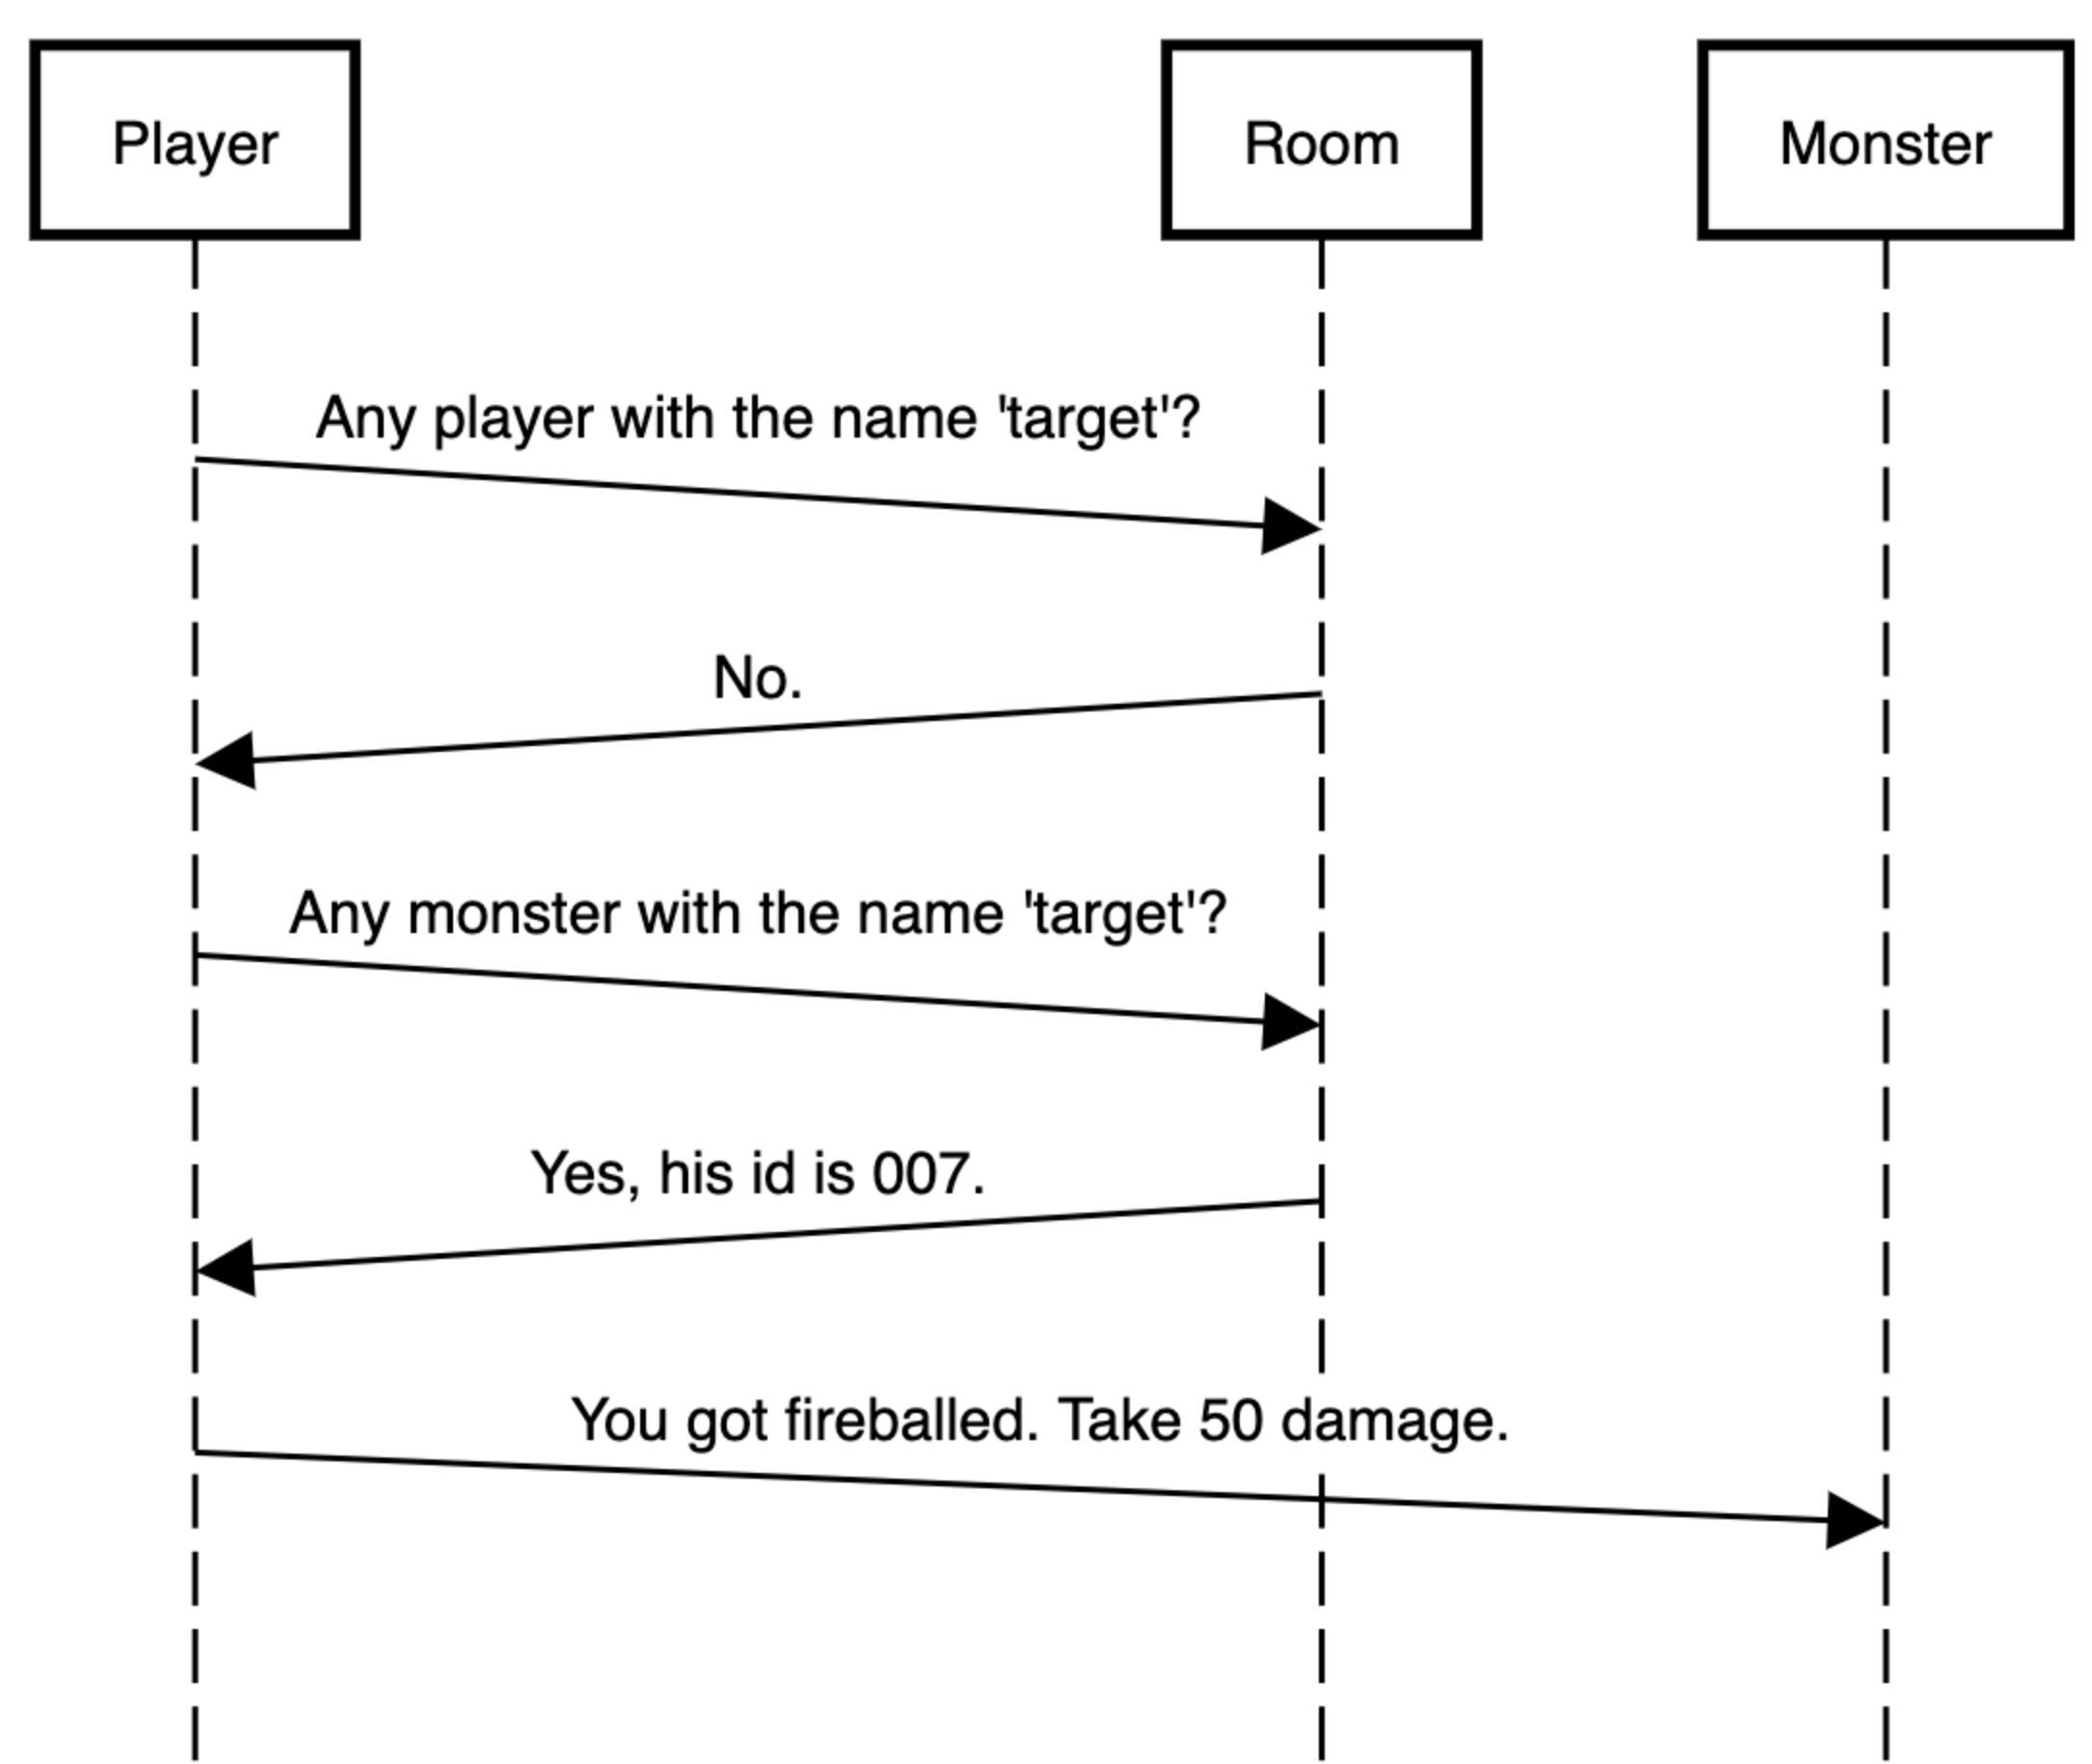
\includegraphics[width=0.7\linewidth]{Materials/Adventuregame/SequenceDiagram}
	\caption{A sequence diagram showing the communication needed for the player to fireball a monster.}
	\label{PLayerFireballFlow}
\end{figure}

As a short introduction to the testing we have done on the adventure game, we would like to provide an overview of the tests done. We have used a table for this, as can be seen in \autoref{tableTests}. The table showcases the number of tests done for each of the unit and integration tests. We will venture deeper into our tests in \autoref{testingDisc}
\begin{table}[H]
	\centering
	\begin{tabular}{| c | c |} \hline
		\textbf{Name} & \textbf{No. of Tests} \\ \hline
		PlayerTests & 30 \\ \hline
		RoomTests & 21 \\ \hline
		WeatherEffectTests & 4 \\ \hline
		BossTests & 4 \\ \hline
		MonsterIntegrationTests & 2 \\ \hline
		PlayerIntegrationTests & 17 \\ \hline
		BossIntegrationTests & 12 \\ \hline
		Total & 90 \\ \hline
	\end{tabular}
	\caption{The number of tests for each grain and connection. Note that this includes tests for all variations, i. e., all abilities and variations are present.}
	\label{tableTests}
\end{table}

\subsection{Metaprogramming} \label{Metalanguage}
We have already talked about what variations are possible to create, but we have not gone into detail about how to achieve them. To create the variation of our adventure game we want, we need a \textit{'reference client'}, a template for what the CLS should be looking for.
\begin{wrapfigure}{L}{0.6\linewidth}
	\vspace{-10px}
	\centering
	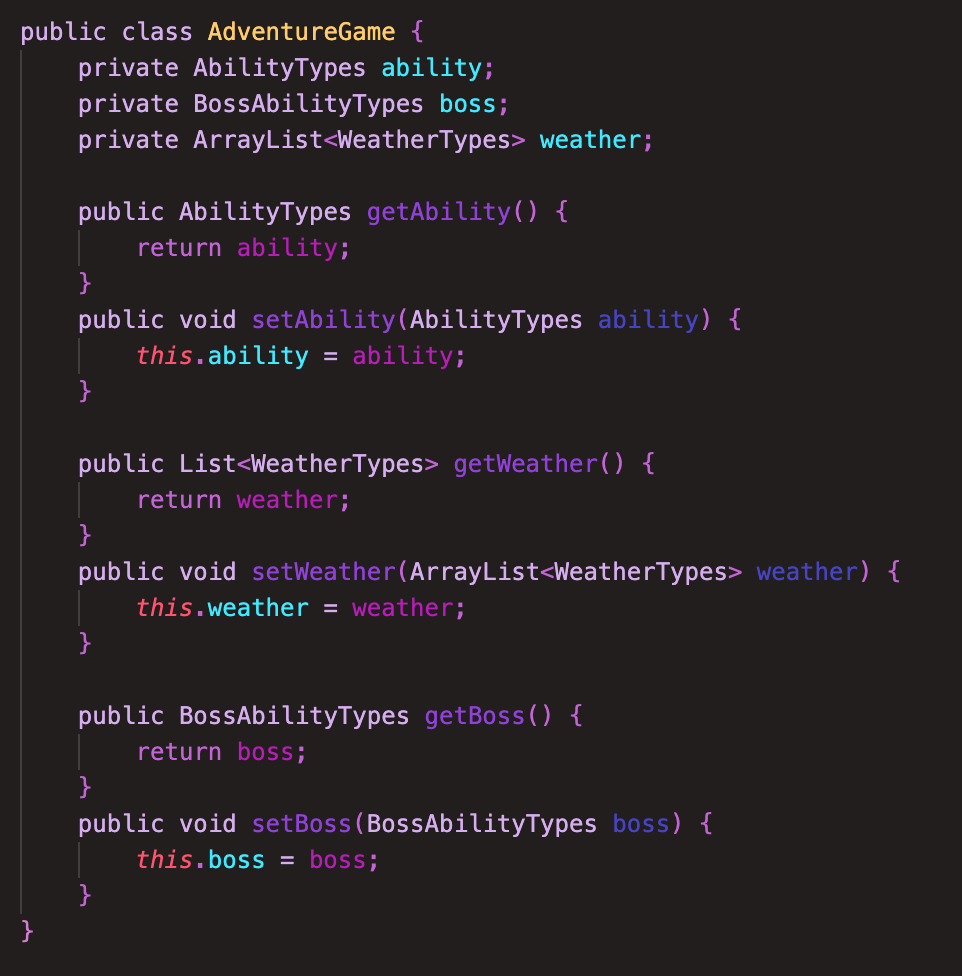
\includegraphics[width=\linewidth]{Materials/Adventuregame/AdventureGame}
	\caption{Super class for adventure games which allows concrete implementations for different variations.}
	\label{MetalanguageAdventure}
\end{wrapfigure} 

To this, we have created a Java class called \textit{AdventureGame} which has methods for setting and getting the player ability, the boss ability and the weather effects. The class can be seen in \autoref{MetalanguageAdventure}. We can inherit from this class to create concrete classes which resemble different variations of our adventure game. We have created several enumerations to hold the possible values for player abilities, boss abilities and weather effects. In \autoref{ConcreteVariation} we can see a variation where the player has the roar ability, the boss has the heal ability and the possible weather effects are blizzard, sunny and cloudy. Only having three different weather effects means that we should only be able to meet these three kinds of weather effects in the game variation, and thus when we talked about randomly selecting a weather type from a pool of available weather effects, we would be able to choose these three weather effects in this variation. Writing the variations in a metalanguage allows to change big parts of the adventure game by writing very few lines of code, making it a very effective way of programming if the code repository for the task is already written.
\begin{figure}[H]
	\centering
	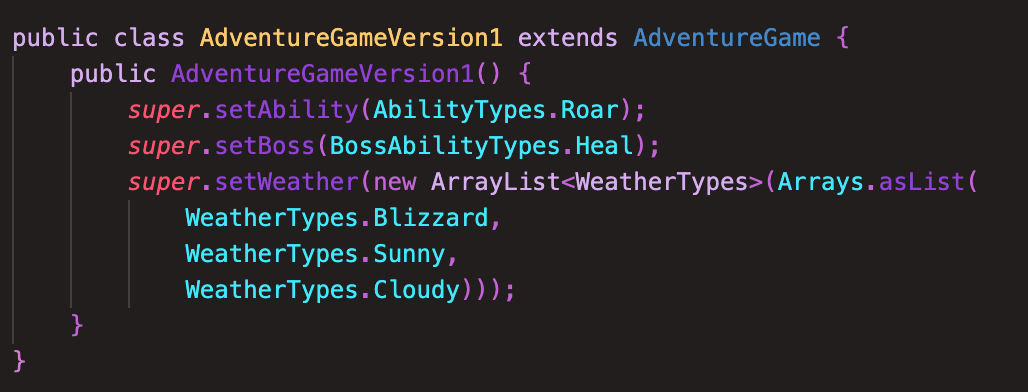
\includegraphics[width=0.8\textwidth]{Materials/Adventuregame/Version1}
	\caption{Concrete implementation of an \textit{AdventureGame}.}
	\label{ConcreteVariation}
\end{figure}

In general the term \textit{metaprogramming} refers to the discipline of writing code which writes code. We here write the Java classes which then with the help of the CLS tool writes the C\# code needed for our adventure game. With the CLS we attach semantic information to each of our combinators such that we with fine granularity can choose the code parts we need. This is a clever way to distinguish code parts which might otherwise just be represented as strings. One could imagine a future where big repositories are created with all sorts of general code and a metalanguage can then be used to speed up development time due to the code already being written, it just needs to be found by a tool like the CLS and be put to use.
